% Introduction to Machine-Learning (1 week)

%\lstinputlisting[language=C++]{src/intro/test.cpp}

The idea behind \emph{supervised machine learning} is to determine a function from a set of training data that can be used to predict the output of new data. The training data is a representative set of examples with input values (typically a vector) and a known output value. Typical machine learning tasks are, for example, \emph{classifications} (discrete output: for example, a molecule is biologically active or not) or \emph{regressions} (continuous output: for example, linear regression).

\begin{center}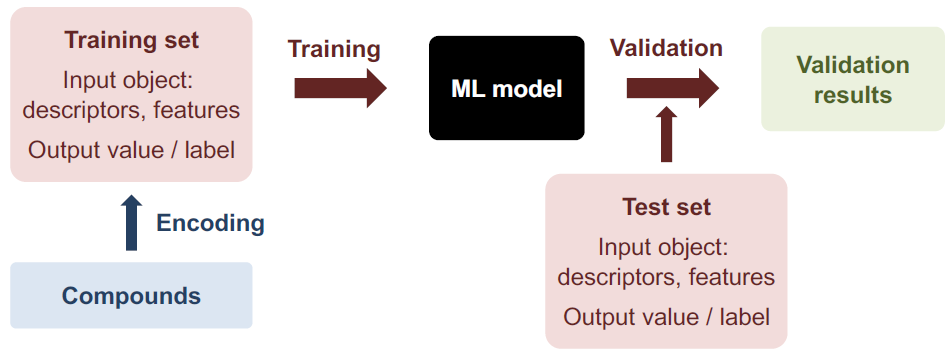
\includegraphics[width=0.65\textwidth]{img/machine/MachineGeneralScheme.png}\end{center}

The following methods, among others, can be used for this purpose:

\begin{itemize}
    \item Linear models, e.g. linear regression, logistic regression
    \item Decision tree
    \item Random forest
    \item Gradient tree boosting
    \item Naïve Bayes
    \item Support vector machines (SVM)
    \item Artificial neural networks
\end{itemize}

\paragraph{Validation}
Once a function has been determined from the training data, it still needs to be validated, since the training data for such algorithms is often too small and there is a risk of overfitting the training data, whereby the function performs well on the training set but not well on new data. Typical validation techniques are \emph{train/test split} or \emph{K-fold cross-validation}.

\begin{center}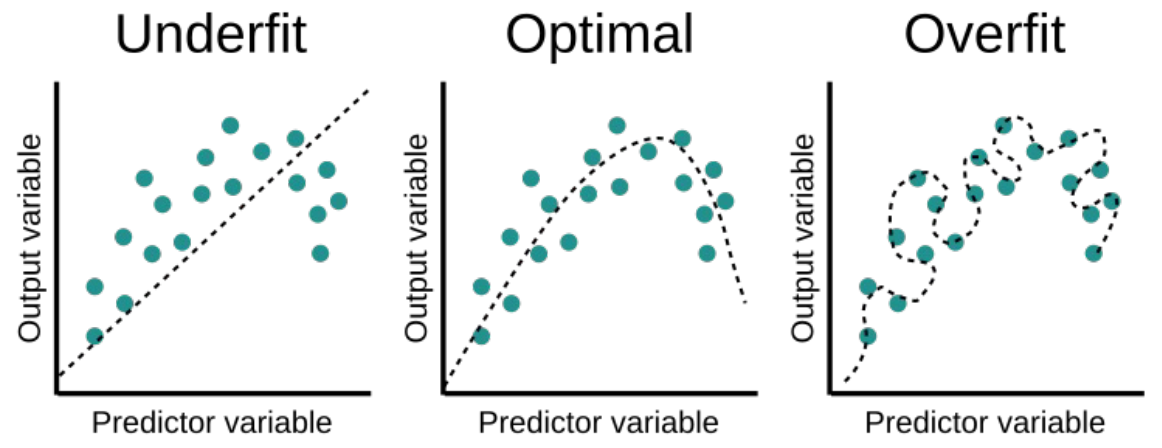
\includegraphics[width=0.65\textwidth]{img/machine/MachineOverUnderFiting.png}\end{center}

For classification models, slightly different assessment criteria for the quality of an ML-model must be applied, such as the \emph{receiver-operator curve} (ROC), in which the true positive rate is plotted against the false positive rate. Depending on the error rates, further metrices for classification models can be calculated.

\begin{center}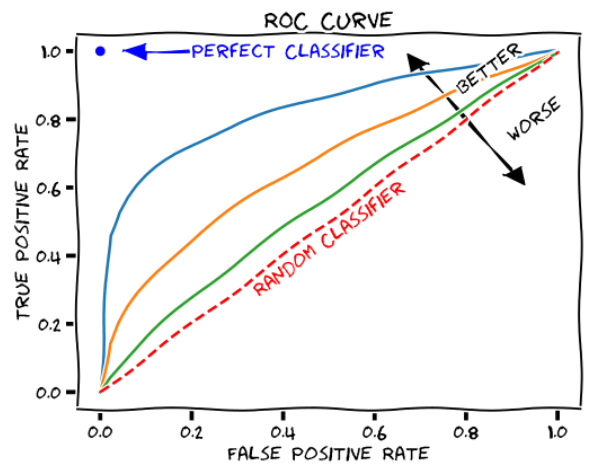
\includegraphics[width=0.45\textwidth]{img/machine/MachineRocCurve.png}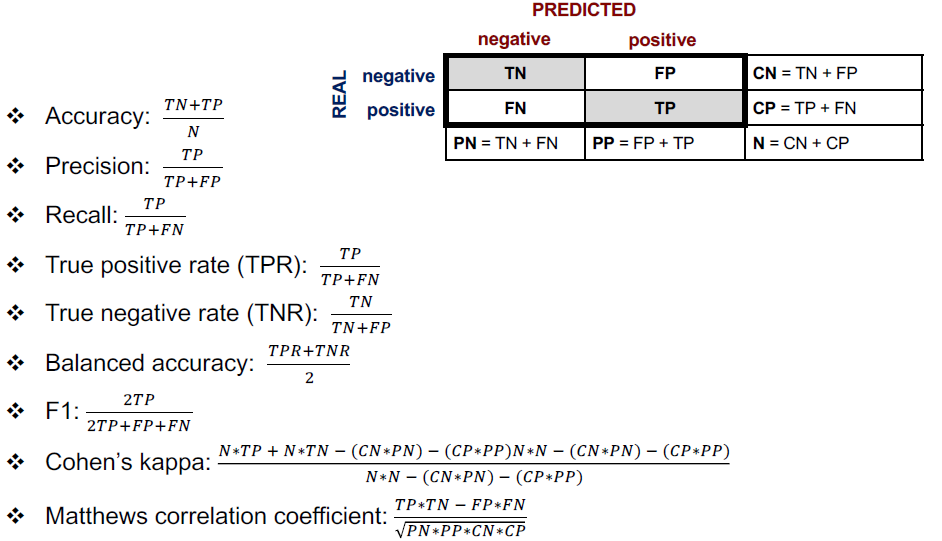
\includegraphics[width=0.45\textwidth]{img/machine/MachineClassificationMetrices.png}\end{center}

\subsection{Linear models: linear regression, logistic regression}



\subsection{Decision trees}

\subsection{Ensemble methods}

\subsection{Artificial neural networks}

\subsection{Practical considerations}